\documentclass[tikz,border=6pt]{standalone}
\usepackage{tikz}
\usetikzlibrary{arrows.meta,positioning}
\definecolor{nebula}{HTML}{6366F1}
\definecolor{spark}{HTML}{14B8A6}
\definecolor{ink}{HTML}{334155}
\begin{document}
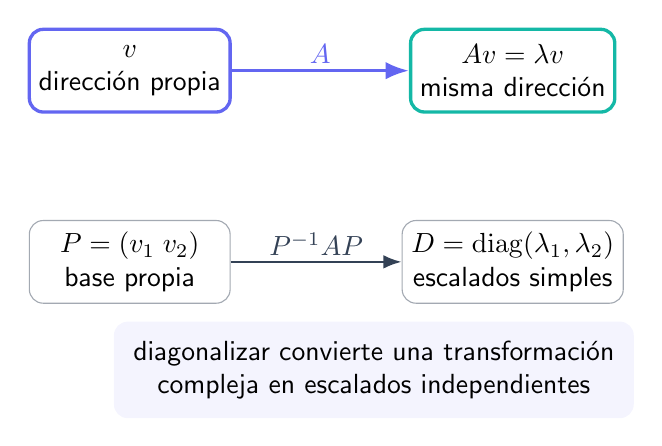
\begin{tikzpicture}[font=\sffamily,>=Latex,box/.style={draw=ink!45,rounded corners=5pt,minimum width=2.55cm,minimum height=1.05cm,align=center,fill=white}]
  \node[box,draw=nebula,very thick] (vector) {$v$\\direcci\'on propia};
  \node[box,right=2.25cm of vector,draw=spark,very thick] (image) {$Av=\lambda v$\\misma direcci\'on};
  \draw[->,very thick,nebula] (vector)--(image) node[midway,above,fill=white,inner sep=2pt] {$A$};
  \node[box,below=1.35cm of vector] (basis) {$P=(v_1\;v_2)$\\base propia};
  \node[box,below=1.35cm of image] (diagonal) {$D=\mathrm{diag}(\lambda_1,\lambda_2)$\\escalados simples};
  \draw[->,thick,ink] (basis)--(diagonal) node[midway,above,fill=white,inner sep=2pt] {$P^{-1}AP$};
  \node[align=center,fill=nebula!7,rounded corners=5pt,inner sep=7pt] at (3.1,-3.8) {diagonalizar convierte una transformaci\'on\\compleja en escalados independientes};
\end{tikzpicture}
\end{document}
